%%%%%%%%%%%%%%%%%%%%%%%%%%%%%%%%%%%%%%%%%%%%%%%%%%%%%%%%%%%%%%%%%%%%%%%%%%%%
% AGUJournalTemplate.tex: this template file is for articles formatted with LaTeX
%
% This file includes commands and instructions
% given in the order necessary to produce a final output that will
% satisfy AGU requirements, including customized APA reference formatting.
%
% You may copy this file and give it your
% article name, and enter your text.
%
% guidelines and troubleshooting are here: 

%% To submit your paper:
\documentclass[draft]{agujournal2019}
\usepackage{url} %this package should fix any errors with URLs in refs.
\usepackage{lineno}
\usepackage{booktabs}
\usepackage{graphicx}
\usepackage{subcaption}
\usepackage{float}

\usepackage[inline]{trackchanges} %for better track changes. finalnew option will compile document with changes incorporated.
\usepackage{soul}
\linenumbers
%%%%%%%
% As of 2018 we recommend use of the TrackChanges package to mark revisions.
% The trackchanges package adds five new LaTeX commands:
%
%  \note[editor]{The note}
%  \annote[editor]{Text to annotate}{The note}
%  \add[editor]{Text to add}
%  \remove[editor]{Text to remove}
%  \change[editor]{Text to remove}{Text to add}
%
% complete documentation is here: http://trackchanges.sourceforge.net/
%%%%%%%

\draftfalse

%% Enter journal name below.
%% Choose from this list of Journals:
%
% JGR: Atmospheres
% JGR: Biogeosciences
% JGR: Earth Surface
% JGR: Oceans
% JGR: Planets
% JGR: Solid Earth
% JGR: Space Physics
% Global Biogeochemical Cycles
% Geophysical Research Letters
% Paleoceanography and Paleoclimatology
% Radio Science
% Reviews of Geophysics
% Tectonics
% Space Weather
% Water Resources Research
% Geochemistry, Geophysics, Geosystems
% Journal of Advances in Modeling Earth Systems (JAMES)
% Earth's Future
% Earth and Space Science
% Geohealth
%
% ie, \journalname{Water Resources Research}

\journalname{Journal of Advances in Modeling Earth Systems (JAMES)}


\begin{document}

%%%%%%%%%%%%%%%%%%%%%%%%%%%%%%%%%%%%%%%%%%%%%%%
%  TITLE
%
% (A title should be specific, informative, and brief. Use
% abbreviations only if they are defined in the abstract. Titles that
% start with general keywords then specific terms are optimized in
% searches)
%
%%%%%%%%%%%%%%%%%%%%%%%%%%%%%%%%%%%%%%%%%%%%%%%

% Example: \title{This is a test title}

\title{Training neural mapping schemes for satellite altimetry with ocean model data}

%%%%%%%%%%%%%%%%%%%%%%%%%%%%%%%%%%%%%%%%%%%%%%%
%
%  AUTHORS AND AFFILIATIONS
%
%%%%%%%%%%%%%%%%%%%%%%%%%%%%%%%%%%%%%%%%%%%%%%%

% Authors are individuals who have significantly contributed to the
% research and preparation of the article. Group authors are allowed, if
% each author in the group is separately identified in an appendix.)

% List authors by first name or initial followed by last name and
% separated by commas. Use \affil{} to number affiliations, and
% \thanks{} for author notes.
% Additional author notes should be indicated with \thanks{} (for
% example, for current addresses).

% Example: \authors{A. B. Author\affil{1}\thanks{Current address, Antartica}, B. C. Author\affil{2,3}, and D. E.
% Author\affil{3,4}\thanks{Also funded by Monsanto.}}

\authors{Q. Febvre\affil{1}, J. Le Sommer\affil{2}, C. Ubelmann\affil{3}, R. Fablet\affil{1}}


% \affiliation{1}{First Affiliation}
% \affiliation{2}{Second Affiliation}
% \affiliation{3}{Third Affiliation}
% \affiliation{4}{Fourth Affiliation}

\affiliation{1}{IMT Atlantique, Lab-STICC, Brest, France}
\affiliation{2}{Université Grenoble Alpes, CNRS, IRD, Grenoble, France}
\affiliation{3}{Datlas, Grenoble, France}
%(repeat as many times as is necessary)


% Corresponding author mailing address and e-mail address:

% (include name and email addresses of the corresponding author.  More
% than one corresponding author is allowed in this LaTeX file and for
% publication; but only one corresponding author is allowed in our
% editorial system.)

% Example: \correspondingauthor{First and Last Name}{email@address.edu}

\correspondingauthor{Quentin Febvre}{quentin.febvre@imt-atlantique.fr}



%%%%%%%%%%%%%%%%%%%%%%%%%%%%%%%%%%%%%%%%%%%%%%%
% KEY POINTS
%%%%%%%%%%%%%%%%%%%%%%%%%%%%%%%%%%%%%%%%%%%%%%%
%  List up to three key points (at least one is required)
%  Key Points summarize the main points and conclusions of the article
%  Each must be 140 characters or fewer with no special characters or punctuation and must be complete sentences

% Example:
% \begin{keypoints}
% \item	List up to three key points (at least one is required)
% \item	Key Points summarize the main points and conclusions of the article
% \item	Each must be 140 characters or fewer with no special characters or punctuation and must be complete sentences
% \end{keypoints}

\begin{keypoints}
\item We propose a simulation-based training approach for the neural mapping of real satellite-derived observations.
\item Simulation-trained neural schemes significantly outperform the operational mapping of real altimetry data for a Gulf Stream case-study.
%\item Learning from ocean simulations and simulated satellite altimetry data produces state-of-the-art mapping performance for real satellite-derived observations. 
\item More realistic simulation datasets improve the performance of the trained neural mapping both quantitatively and qualitatively. 
%\item Two ways to obtain more realistic synthetic data are increasing the resolution of the numerical simulation and model reanalysis.
\end{keypoints}

%%%%%%%%%%%%%%%%%%%%%%%%%%%%%%%%%%%%%%%%%%%%%%%
%
%  ABSTRACT and PLAIN LANGUAGE SUMMARY
%
% A good Abstract will begin with a short description of the problem
% being addressed, briefly describe the new data or analyses, then
% briefly states the main conclusion(s) and how they are supported and
% uncertainties.

% The Plain Language Summary should be written for a broad audience,
% including journalists and the science-interested public, that will not have 
% a background in your field.
%
% A Plain Language Summary is required in GRL, JGR: Planets, JGR: Biogeosciences,
% JGR: Oceans, G-Cubed, Reviews of Geophysics, and JAMES.
% see http://sharingscience.agu.org/creating-plain-language-summary/)
%
%%%%%%%%%%%%%%%%%%%%%%%%%%%%%%%%%%%%%%%%%%%%%%%

%% \begin{abstract} starts the second page

\begin{abstract}
  The absence of reference data, which defines the expected model outputs, poses a challenge when training machine learning models with Ocean observations. Here, we put forward the idea that leveraging both simulated observations and ocean quantities for learning purposes provides a powerful method to develop real-world applications.
  For example, we focus here on the problem of satellite altimetry interpolation which consist in reconstructing the dynamic field of sea surface height (SSH) from satellite observations that have a high rate of missing data and irregular sampling. Data-driven models have been successfully demonstrated for this task in supervised settings using an observation simulated system experiment (OSSE), i.e. with a simulated SSH field as learning target and pseudo-observations as inputs.
  However the learning paradigm used in those demonstrations can not be trivially transferred to real altimetry observations by lack of knowledge of the true SSH field.
  We ask here if and under what condition the knowledge extracted from synthetic data transfers to real observations. We study the impact of the ocean run resolution, observation data reanalysis and of explicit tide modeling on training an interpolator over the Gulfstream region. We find that the different datasets reliably offers better performance than the current operational product DUACS when evaluated on real altimetry data. Additionally, a more realistic ocean simulation through higher resolution or model reanalysis has been shown to be significant factors for achieving better reconstruction performance on our test case. Our best model improves the longitudinal scale resolved from 152 kilometers for DUACS to 98 kilometers and improves the root mean squared error (RMSE) by 28\%.
  We believe that this work opens interesting perspectives for developing synergies between ocean modeling and operational product development by leveraging learning based approaches.

\end{abstract}

\section*{Plain Language Summary}

% https://www.agu.org/Share-and-Advocate/Share/Community/Plain-language-summary
In order for an artificial intelligence to learn, one need to describe a task using data and an evaluation procedure. For example, to train a model to recognize trees, one need pictures of trees and the labels of the type of tree in the pictures to evaluate and train the model.
For some problems we have access to a lot of data but cannot easily train a model because we can't evaluate it on the task of interest. This happens in ocean science where a lot of instruments gather observation data but it's not always easy to compute what the model should be trained for.
Here we look at a specific task which is to construct images related to the ocean surface currents from what satellites can see. The satellite data we're using can be seen as an image of the ocean surface with a lot of missing data (~95\% of missing pixels for a given day), and we would like to train an artificial intelligence to find the values of the missing pixels.
As described before, when our model fills the gaps a certain way, we cannot easily say how good is the reconstruction because we don't precisely know what the values should be. And it is therefore challenging to train such an artificial intelligence using only the satellite data.
However, scientists know a lot about the ocean, how the currents behave and they're able to simulate fake oceans in big computers. Using these fake oceans, we can train A.I. models to fill the gaps by first hiding some pixels and checking if the model gives the correct values for the hidden data.
In this paper we explore if A.I.s trained on fake oceans are useful for the real ocean and study what is the best fake ocean for training an A.I. .
We show that today's fake oceans work well for training an A.I. and that the best way to obtain a great A.I. is to use a fake ocean that has been simulated with a higher resolution!

%%%%%%%%%%%%%%%%%%%%%%%%%%%%%%%%%%%%%%%%%%%%%%%
%
%  BODY TEXT
%
%%%%%%%%%%%%%%%%%%%%%%%%%%%%%%%%%%%%%%%%%%%%%%%

%%% Suggested section heads:
% \section{Introduction}
%
% The main text should start with an introduction. Except for short
% manuscripts (such as comments and replies), the text should be divided
% into sections, each with its own heading.

% Headings should be sentence fragments and do not begin with a
% lowercase letter or number. Examples of good headings are:

% \section{Materials and Methods}
% Here is text on Materials and Methods.
%
% \subsection{A descriptive heading about methods}
% More about Methods.
%
% \section{Data} (Or section title might be a descriptive heading about data)
%
% \section{Results} (Or section title might be a descriptive heading about the
% results)
%
% \section{Conclusions}


\section{Introduction}


% ML pour traitement de données satellite, bcp d'applications recentes 

% en particulier tache de gap-filling et cartoigraphie 

% un bon exemple altimétrie, methodes expertes et methodes methodes basées données. 

%--- [difficulté : suprenante, pas vraiment assez de données pour entrainer algo complexe (millions partame) [en fait non]]

% algo basé donnée : modele parametrique (calibration faible nombre de params : MIOST, DYNMOST), algo issue du DL (grnd nombre de param, NN expressif, peu d'hypothese)

% algo DL, besoin de bcp de données, en prqtique, peuvent entrainée sur données modeles. ex papier de SEATTLE. (emergence : modele numerique pour ca.) 

% question comment se fait le tranfert, sous quelle condition un lodele est-il bon poru entrainer algo pour tache donées reel. 

% Dans cet article, on demontre que modele peut marcher, cas particuler altimétrie, influence de la donnée d'entrée 

% le plan de l'artle, c'est ca 


% at least 3 paragrapghs:
  %Ocean processes are complex, difficult to model and expensive to simulate. On the other hand, ocean research usually involves very large amount of data, either from ocean simulation outputs or from observing systems. This motivates the research into learning based methods that are able to extract knowledge from the available data.

  % proposition d'intro centrée altimétrie
  % possibilité d'une intro plus générique avec un cas d'étude altimétrie (mais moins en phase sur la partie résultat/conclusion altimétrie?)
  Satellite altimeters have brought a great leap forward in the observation of sea surface height on a global scale since the 80's. They have greatly contributed to the monitoring and understanding of key processes such as the rise of the mean ocean level due to rising temperature and the role of mesoscale dynamics. The retrieval of mesoscale-to-submesoscale sea surface dynamics for horizontal scales smaller than 150 km however remains a challenge for operational systems based on optimal interpolation \cite{taburetDUACSDT2018252019} and data assimilation \cite{jean-michelCopernicusGlobal122021} schemes. This has motivated a wealth of research to develop novel mapping schemes \cite{ballarottaDynamicMappingAlongTrack2020,ubelmannReconstructingOceanSurface2021,guillouMappingAltimetryForthcoming2021}.

  In this context, data-driven and learning-based approaches \cite{alveraazcarateReconstructionIncompleteOceanographic2005,barthDINCAEMultivariateConvolutional2022,lguensatAnalogDataAssimilation2017,fabletENDTOENDPHYSICSINFORMEDREPRESENTATION2021,martinSynthesizingSeaSurface2023} appear as appealing alternatives to make the most of the available simulation and observation datasets. Especially, Observing System Simulation Experiments (OSSE) have stressed the potential of the supervised learning of neural schemes for the mapping of satellite-derived altimetry data \cite{fabletENDTOENDPHYSICSINFORMEDREPRESENTATION2021,beauchamp4DVarNetSSHEndtoendLearning2023}. Their applicability to real datasets has yet to be assessed and recent studies have rather explored unsupervised learning strategies from real gappy multi-year altimetry datasets \cite{martinSynthesizingSeaSurface2023}. Despite promising results, these schemes do not reach the relative improvement of the operational processing suggested by OSSE-based studies.   
  
Here, we go beyond the exploitation of OSSE as benchmarking-only testbeds. We explore their use for the training of neural mapping schemes which we apply to real altimetry dataset. Through numerical experiments on a Gulf Stream case-study for 2003-2005 4-nadir altimeter constellation, our key contributions are as follows:  
%  Conversely some processes such as the mesoscale to sub-mesoscale currents of horizontal scales smaller than 150 km are yet to be well reconstructed from the altimeter's observations due to the scarce and irregular sampling. Resolving those scales would greatly benefit climate monitoring since the dynamics at those scales play a key role in ocean/atmosphere exchange.
  %Data-driven approaches such as the 4DVarNet have shown their potential to outperform current operational approaches and resolve scales below 100km in OSSE setups. Although those results are promising, the training and evaluation were made on simulated data, thus there are no guaranties that they hold true when working with real observation data.
  %Whereas some works try to design a training procedure on observation data, we ask whether a training done on synthetic data can be transferred to real application and under what conditions.
  % The transfer learning problem address this question on whether a knowledge gained on a specific task (reconstructing a simulated field) will be applicable to an other (reconstructing the ocean state) and has been .
%    Our main contributions are as follows:
    \begin{itemize}
    \item{We demonstrate the relevance of the supervised OSSE-based learning of neural mapping schemes for the space-time interpolation of real nadir altimetry data;}
    \item{We benchmark the proposed approach with state-of-the-art operational products as well as neural schemes trained from real altimetry datasets;}    
    \item{We benchmark neural schemes trained with the proposed OSSE-based strategy using different simulation datasets and we assess the impact of the characteristics of these datasets on the mapping performance.}
%    Demonstrate numerically that today's numerical simulations of the ocean are a valuable resource for training machine learning models to be applied on real data, with added benefit of more realistic synthetic data}
    \end{itemize}
To ensure the reproducibility of our results, our code is made available through an open source license along with the considered datasets and the trained models.

    
The content of this paper is organized in the following manner. Section \ref{sec:background} offers background information on related work, Section \ref{sec:method} presents our method, Section \ref{sec:results} reports our numerical experiments, and Section \ref{sec:conclusion} elaborates on our main contributions.
%Text here ===>>>


\section{Background}
\label{sec:background}
\subsection{Satellite altimetry gridded products}
\label{ssec:interpolation}
The mapping of altimetry data to produce gridded products is a necessary step to observe surface dynamics.

Three classes of approaches have emerged over the years. 

Data assimilation products using large ocean models such as the GLORYS12 reanalysis \cite{jean-michelCopernicusGlobal122021}.This approach leverage the full expressiveness of state of the art ocean models and aims at generating trajectories close to observed quantities through data assimilation methods such as Kalman filtering\cite{} and four dimensional variational data assimilation (4DVAR)\cite{carrassiDataAssimilationGeosciences2018}.

Observation products made with little dynamical assumptions such as optimal interpolation products such as DUACS which is today operational product \cite{taburetDUACSDT2018252019} or Back and forth nudging using simplified quasi-geostrophic dynamics (BFNQG) as described in \cite{guillouMappingAltimetryForthcoming2021}

Data driven interpolation schemes recently gained momentum using machine learning techniques or parameterized formulations calibrated on historical observation data.\cite{alveraazcarateReconstructionIncompleteOceanographic2005,fabletENDTOENDPHYSICSINFORMEDREPRESENTATION2021,ubelmannReconstructingOceanSurface2021}


%For the last decades nadir satellite altimeters have orbited the earth and have provided oceanographers with an unprecedented coverage of the ocean surface topography. Indeed, a constellation of 4 to 7 satellites acquired one dimensional profiles globally. However, in order to study the observe the surface currents, one need to observe the gradients of the surface topography which brings in the necessity for producing a gridded product from nadir altimetry tracks.


% We can distinguish three classes of approaches for generating SSH gridded products:
% \begin{itemize}
%     \item Data assimilation products using large ocean models such as the GLORYS12 reanalysis \cite{jean-michelCopernicusGlobal122021}
%     \item Observation products made with little dynamical assumptions that are calibrated on observation data \cite{taburetDUACSDT2018252019,guillouMappingAltimetryForthcoming2021} 
%     \item Data driven interpolation schemes \cite{alveraazcarateReconstructionIncompleteOceanographic2005,fabletENDTOENDPHYSICSINFORMEDREPRESENTATION2021,ubelmannReconstructingOceanSurface2021}
% \end{itemize}


\subsection{Ocean Modeling and OSSE}
\label{ssec:oceanmodeling}
Efforts in modeling and simulating ocean physics have been essentials for better understanding the processes involved in the earth system and being able to project future behaviours \cite{bernardImpactPartialSteps2006,ajayiSpatialTemporalVariability2020}. 
High resolution simulations used in Observing System Simulation Experiments (OSSE) also provide a great test-bed for developing and evaluating new ways observing the ocean. For example, in the case of the recently launched SWOT mission, a novel instrument has been deployed and the calibration methods were developed and evaluated using ocean and instrument simulations\cite{}. 
The development of methods for interpolating altimetry tracks such as the BFNQG and 4DVarNet are also traditionally demonstrated in OSSE setup for ease of evaluation before being considered for real data use. 

%However the use of ocean models for observation data reanalysis presents some challenges. The computational cost of running ocean physics limits the model used either in the range processes modeled or in the resolution at which the model is ran. 
%Additionally when looking at the reconstruction error and the scales effectively resolved along an altimetry tracks, we find that a reanalysis such as GLORYS12 performs significantly worse than an optimal interpolation product like DUACS.


\subsection{Physics-aware deep-learning}
\label{ssec:deeplearning}
In the last decades, machine learning advances combined with the rise in compute power and amount of data have shown the power of extracting knowledge from data in a variety of domains ranging from computer vision to language processing. 
However one fundamental limitation of learning from data is the bad generalization performance outside the the training distribution. This is of critical importance for physical systems, where training a learning-based model on past data will seldom perform well when the system evolves and reaches dynamics absent from the training data. We can see evidence of this shortcoming in the instability challenges faced by neural closures for climate models \cite{brenowitzInterpretingStabilizingMachineLearning2020}. 
On the flip side, physical laws grant practically unlimited capacity for generalization in any given scenario, yet they fall short of fully capitalizing on the knowledge embedded in the accessible data.

There have been a variety of approaches trying to harness the best of both world. Some injecting trainable components in classical integration scheme of physical model such as Yin et al. \cite{yinAugmentingPhysicalModels2021b}, other leveraging physical prior within their learning setups. The physical prior has been used in the training objective \cite{raissiPhysicsinformedNeuralNetworks2019,greydanusHamiltonianNeuralNetworks2019}, as well as in the architecture \cite{li2020fourier,Wang2020TF}.

However most of these works have focused on relatively simple physical models and it remains challenging to combine current state of the art ocean models with such methods due to the complexity and cost of running the physical model, the differences in languages and infrastructure used in each domain, as well the difficulty (if not impossibility) of computing the gradients of an integration step of the ocean model.

In this paper we would like to push for the idea that a great way to benefit from the advances made by the ocean modeling community is to use high-resolution runs of ocean models as training data to learn deep neural model for ocean reanalysis. 


\subsection{Synthetic data training and transfer learning}
\label{ssec:transferlearning}
Machine learning practitioners often face a significant challenge of limited annotated data when training supervised learning schemes, and creating large annotated datasets for a given task can be expensive or infeasable.
Prior research efforts have effectively tackled this issue by either leveraging existing related annotated datasets \cite{dengImageNetLargescaleHierarchical2009} or generating synthetic data\cite{gomezgonzalezVIPVortexImage2017,dosovitskiyFlowNetLearningOptical2015}.
The model trained on those related dataset can then be transferred to the relevant task given that the training data manages to capture the true distribution of the target situations.

In ocean science recent work have used simulation data to train super-resolution model of the SSH \cite{buongiornonardelliSuperResolvingOceanDynamics2022} and our work aims to further investigate the potential of such training schemes. 


\section{Method}
\label{sec:method}
%
\begin{figure}[H]
    \centering
    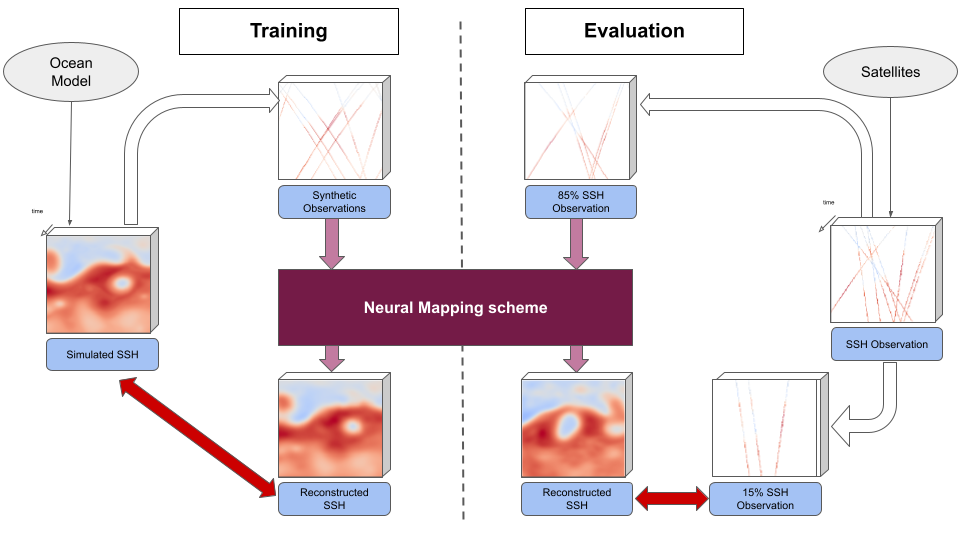
\includegraphics[width=\textwidth]{figures/schema_method.png}
    \caption{Overview of the experimental setup. On the left side we display the OSSE training principle based on an ocean simulation which will be used for 1) generating synthetic observation and 2) the training objective of the neural mapping scheme. On the right side we show the evaluation principle of splitting the available satellite observations to evaluate the method on data that were not used for the inference.}
    \label{fig:method}
\end{figure}
\subsection{Overview}
\label{ssec:overview}
\begin{figure}[ht]
    \centering
    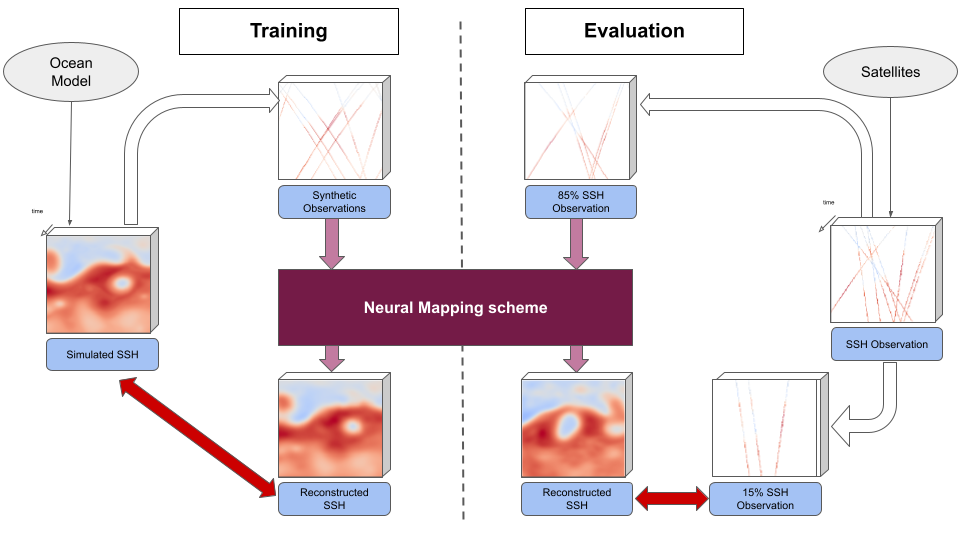
\includegraphics[width=\textwidth]{figures/schema_method.png}
    \caption{Overview of the experimental setup. On the left side we display the OSSE training principle based on an ocean simulation which will be used for 1) generating synthetic observation and 2) the training objective of the neural mapping scheme. On the right side we show the evaluation principle of splitting the available satellite observations to evaluate the method on data that were not used for the inference.}
    \label{fig:method}
\end{figure}
In this section, we describe the method used to evaluate the impact of the choice of synthetic SSH data for training a altimetry mapping algorithm. We first describe the architecture trained, as well as the different sources of SSH data that were evaluated. And the describe the training and evaluation procedure used.

\subsection{Model}
\label{ssec:4dvarnet}
We consider the 4DVarNet model for our study. It's a variational data assimilation method where the prior cost formulated using a physically-aware convolutional neural network, and the minimization procedure is done using a ConvLSTM network in a fashion inspired from the Learning to learn paper.
The overall architecture and components are the same as the one described in previous publications. Some changes in the implementation details have been made that were found to empirically improve the performance and reduce the training time. We refer the reader to the code for more details.


\subsection{SSH Data}

\label{ssec:data}

\begin{table}[h]
    \centering
\begin{tabular}{|l||cccc|}
\toprule
{} & Resolution & Reanalysis & Tide & DAC  \\
\midrule
NATL60 \cite{ajayiSpatialTemporalVariability2020}               &      1/60 $^\circ$ &               No &            No &                   No  \\
eNATL60-t \cite{brodeauOceannextENATL60Material2020}         &      1/60 $^\circ$ &               No &           Yes &                  Yes  \\
eNATL60-0 \cite{brodeauOceannextENATL60Material2020}         &      1/60 $^\circ$ &               No &            No &                  Yes  \\
GLORYS12-r \cite{jean-michelCopernicusGlobal122021} &      1/12 $^\circ$ &              Yes &            No &                   No  \\
GLORYS12-f \cite{jean-michelCopernicusGlobal122021}   &      1/12 $^\circ$ &               No &            No &                   No  \\
ORCA025 \cite{bernardImpactPartialSteps2006}             &       1/4 $^\circ$ &               No &            No &                   No  \\
\bottomrule
\end{tabular}
\caption{Summary table of the synthetic data tested for training}
\label{tab:data}
\end{table}

Digital ocean models are intricate software programs that incorporate numerous configuration parameters. In order to better isolate influence factors, we considered different outputs from the NEMO ocean model ran with different configurations. We selected six distinct datasets, enabling us to examine the influence of three factors on the dynamical structures manifested in the simulations.
In order to evaluate the impact of the grid resolution at which the model is ran we consider the runs ORCA025, NATL60 and the free run of GLORYS12 (F12) which are respectively run at 1/4°, 1/60°, 1/12°. We know that finer grids allow for more processes to be simulated. We expect dynamics to therefore be closer to the real ocean in higher resolution simulation and a deep learning approach that has been trained on more faithful dynamics to perform better.
Another way to nudge ocean simulations to more realistic dynamics is by assimilating observation data. To evaluate this aspect we compare the GLORYS12 reanalysis and its associated the free run. Measurements of temperature, sea level, sea ice concentration and salinity have been assimilated during the reanalysis.
Finally the recent eNATL twin simulations offers another point of comparison which is the impact of the presence or absence of explicit modeling of tide motion in the simulation.
Overall those datasets provide different ways to study the impact of the dynamics present and it should be noted that the computational cost of producing these dataset is intricately linked to the range of processes that are expressed whether it's thanks to the grid resolution, reanalysis or explicit modeling.


\subsection{Training and Evaluation}
\label{ssec:training}
In order to fairly evaluate the datasets' quality as a training resource, we strive to standardize as many other training aspects as possible.
All simulations are regridded to the same resolution (1/20°) and daily averages are used as training target. We generate the noise-free pseudo-observations by sampling values of the daily averages corresponding to realistic orbits of a 5 altimeters-constellation. All models are trained using one-year synthetic dataset in a domain around the Gulfstream from (66°W, 32°N) to (54°W, 44°N) in which the same two-months are kept for validation. The hyper-parameters of the model and training procedure such as the number of epoch, learning rate scheduler are the same for each experiments. The models are trained on reconstructing the SSH fields and the amplitude of the gradients as well as a regularization cost on the prior model.

The evaluation is done using altimetry data from the 6 satellites constellation of 2017. Five satellites are used as inputs for the mapping and one is kept out for computing the metrics. The metrics results from interpolating the gridded product on the altimetry tracks  over the domain from (65°W, 33°N) to (55°W, 43°N) and computing the metrics in the along-track geometry. This setup is standardized in a data-challenge where different methods have been compared on two metrics: $\mu$ a root mean squared error (RMSE) normalized by the variance of the SSH signal at each location and a spectral score called effective scale resolved corresponding to the wave-number where the power spectrum density (PSD) of the error is half the one of the SSH signal.   

\begin{figure}[H]
\small
\begin{center}
\setlength{\tabcolsep}{1pt}
\begin{tabular}{ccccc}
 &&
&\hspace{-30mm} 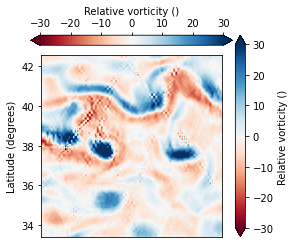
\includegraphics[trim={8mm 7cm 22mm 0},clip,width=3.0cm,height=0.7cm]{figures/plots/horizontal_cbar_vort.png} &\\
\hspace{0mm} &&
\hspace{-30mm} Training  
\hspace{3mm}  & 
 & 
\hspace{-30mm} Reconstruction \\

%\vspace{-2mm}
%%%%% ORCA025 %%%%%%%%

\hspace{-10mm}  1)&
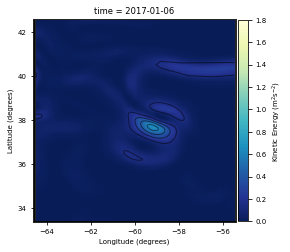
\includegraphics[trim={0 13mm 22mm 5mm},clip, width=3.3cm,height=2.9cm]{figures/plots/orca025_train_ke.png} &
 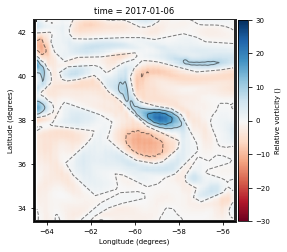
\includegraphics[trim={13mm 13mm 22mm 5mm},clip, width=2.9cm,height=2.9cm]{figures/plots/orca025_train_vort_r.png} &
 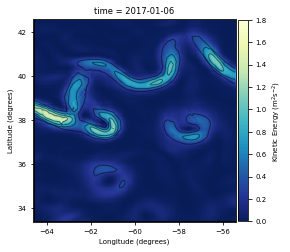
\includegraphics[trim={13mm 13mm 22mm 5mm},clip, width=2.9cm,height=2.9cm]{figures/plots/orca025_rec_ke.png} &
 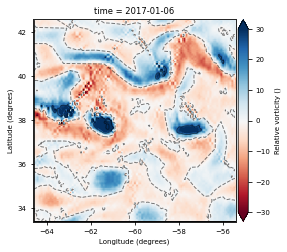
\includegraphics[trim={13mm 13mm 22mm 5mm},clip,width=2.9cm,height=2.9cm]{figures/plots/orca025_rec_vort_r.png} \\
%\vspace{3mm}
%%%%% GLORYS12-f %%%%%%%%
\hspace{-10mm} 2) &
 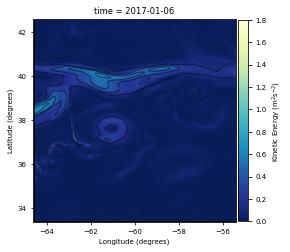
\includegraphics[trim={0 13mm 22mm 5mm},clip, width=3.3cm,height=2.9cm]{figures/plots/glorys12-f_train_ke.png} &
 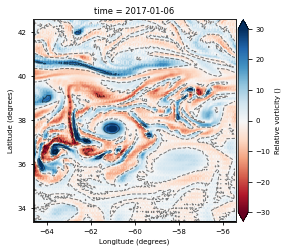
\includegraphics[trim={13mm 13mm 22mm 5mm},clip, width=2.9cm,height=2.9cm]{figures/plots/glorys12-f_train_vort_r.png} &
 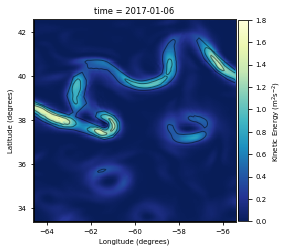
\includegraphics[trim={13mm 13mm 22mm 5mm},clip, width=2.9cm,height=2.9cm]{figures/plots/glorys12-f_rec_ke.png} &
 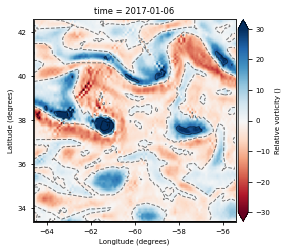
\includegraphics[trim={13mm 13mm 22mm 5mm},clip,width=2.9cm,height=2.9cm]{figures/plots/glorys12-f_rec_vort_r.png} \\
%\vspace{3mm}
%%%%% GLORYS12-f %%%%%%%%
\hspace{-10mm} 3) &
 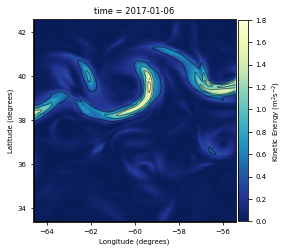
\includegraphics[trim={0 13mm 22mm 5mm},clip, width=3.3cm,height=2.9cm]{figures/plots/glorys12-r_train_ke.png} &
 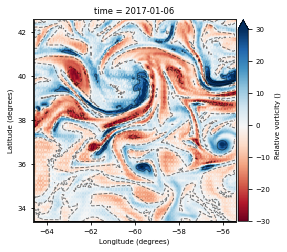
\includegraphics[trim={13mm 13mm 22mm 5mm},clip, width=2.9cm,height=2.9cm]{figures/plots/glorys12-r_train_vort_r.png} &
 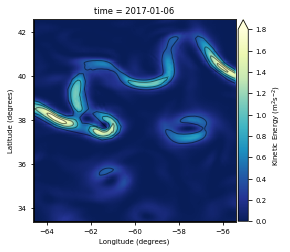
\includegraphics[trim={13mm 13mm 22mm 5mm},clip, width=2.9cm,height=2.9cm]{figures/plots/glorys12-r_rec_ke.png} &
 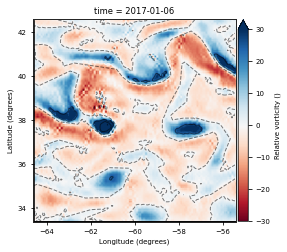
\includegraphics[trim={13mm 13mm 22mm 5mm},clip,width=2.9cm,height=2.9cm]{figures/plots/glorys12-r_rec_vort_r.png} \\
%%%%% NATL60 %%%%%%%%
\hspace{-10mm} 4) &
 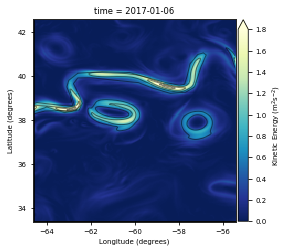
\includegraphics[trim={0 13mm 22mm 5mm},clip, width=3.3cm,height=2.9cm]{figures/plots/natl60_train_ke.png} &
 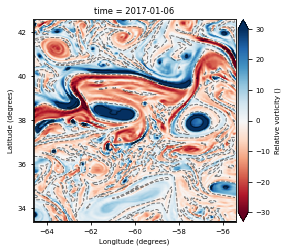
\includegraphics[trim={13mm 13mm 22mm 5mm},clip, width=2.9cm,height=2.9cm]{figures/plots/natl60_train_vort_r.png} &
 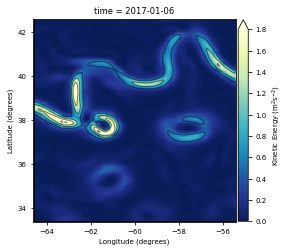
\includegraphics[trim={13mm 13mm 22mm 5mm},clip, width=2.9cm,height=2.9cm]{figures/plots/natl60_rec_ke.png} &
 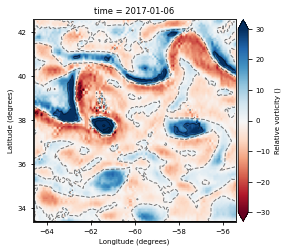
\includegraphics[trim={13mm 13mm 22mm 5mm},clip,width=2.9cm,height=2.9cm]{figures/plots/natl60_rec_vort_r.png} \\
%\vspace{3mm}
%%%%% eNATL60-t %%%%%%%%
\hspace{-10mm} 5) &
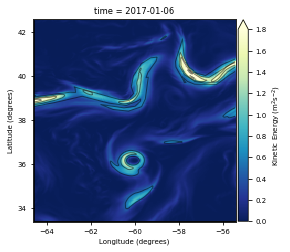
\includegraphics[trim={0 13mm 22mm 5mm},clip, width=3.3cm,height=2.9cm]{figures/plots/enatl60-t_train_ke.png} &
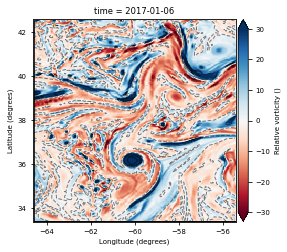
\includegraphics[trim={13mm 13mm 22mm 5mm},clip, width=2.9cm,height=2.9cm]{figures/plots/enatl60-t_train_vort_r.png} &
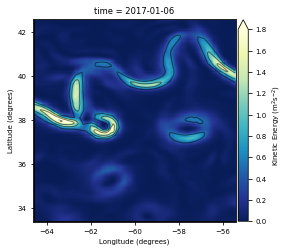
\includegraphics[trim={13mm 13mm 22mm 5mm},clip, width=2.9cm,height=2.9cm]{figures/plots/enatl60-t_rec_ke.png} &
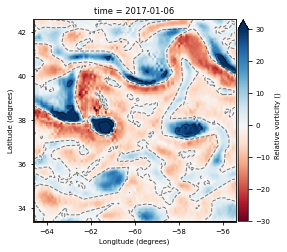
\includegraphics[trim={13mm 13mm 22mm 5mm},clip,width=2.9cm,height=2.9cm]{figures/plots/enatl60-t_rec_vort_r.png} \\
%\vspace{3mm}
%%%%% eNATL60-0 %%%%%%%%
\hspace{-10mm} 6) &
 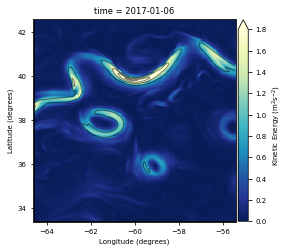
\includegraphics[trim={0 0 19mm 5mm},clip, width=3.3cm,height=3.1cm]{figures/plots/enatl60-0_train_ke.png} &
 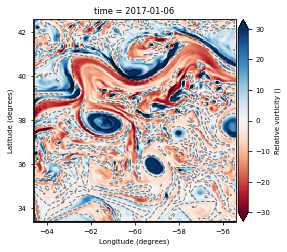
\includegraphics[trim={13mm 0 22mm 5mm},clip, width=2.9cm,height=3.1cm]{figures/plots/enatl60-0_train_vort_r.png} &
 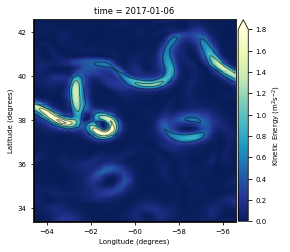
\includegraphics[trim={13mm 0 22mm 5mm},clip, width=2.9cm,height=3.1cm]{figures/plots/enatl60-0_rec_ke.png} &
 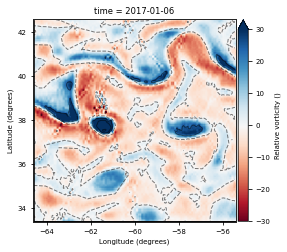
\includegraphics[trim={13mm 0 22mm 5mm},clip,width=2.9cm,height=3.1cm]{figures/plots/enatl60-0_rec_vort_r.png} \\
 \hspace{-15mm} &(a) & (b) & (c) & (d) \\
 &&
&\hspace{-30mm} 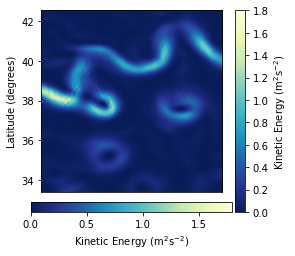
\includegraphics[trim={8mm 0 22mm 7cm},clip,width=2.5cm,height=0.7cm]{figures/plots/horizontal_cbar_ke_bottom.png} &\\
% \vspace{-2mm}

\end{tabular}
\vspace{-3mm}
% \caption{Row I - Isotrophic PSD. Row 2 - Isotrophic PSD Score}
\caption{
Kinetic energy ((a) and (c) and relative vorticity ((b) and (d)) of the training dataset ((a) and (b)) and the associated 4DVarNet reconstructions ((c) and (d)) at the 6th of January of their respective year.
Each row shows the experiment using: 1) ORCA025, 2) GLORYS12-f, 3) GLORYS12-r, 4) NATL60, 5) eNATL60-t, 6) eNATL60-0}
\vspace{-5mm}
\label{fig:maps}
\end{center}
\end{figure}

\section{Results}
\label{sec:results}





\subsection{Benchmarking results}
\label{ssec:benchmarks}

\begin{table}[h!]
\centering
\begin{tabular}{|l||llll|rrr|}
\toprule
 & SSH  & Deep  & Calibrated on  & Physical  & rmse & $\mu_{ssh}$  & $\lambda_x$ \\
 &  Only &  Learning &  data from &  Model &  (cm) &  () &  (km) \\
\midrule
(a) 4DVarNet &  Yes & Yes & Simulation  & None & 5.9  & 0.91  & 98 \\
(b) MUSTI & No &  Yes & Satellite  & None & 6.3  & 0.90  & 112 \\
(c) ConvLstm-SST & No &  Yes & Satellite  & None & 6.7  & 0.90  & 108 \\
(d) ConvLstm &  Yes &  Yes & Satellite  & None & 7.2  & 0.89  & 113 \\
(e) DYMOST&  Yes & No & Satellite  & QG & 6.7  & 0.90  & 131 \\
(f) MIOST &  Yes & No & Satellite  & None & 6.8  & 0.90  & 135 \\
(g) BFN-QG &  Yes & No & Satellite  & QG & 7.6  & 0.89  & 122 \\
(h) DUACS &  Yes & No & Satellite  & None & 7.7  & 0.88  & 151 \\
(i) GLORYS12 & No & No & Satellite  & NEMO & 15.1  & 0.77  & 241 \\
\bottomrule
\end{tabular}
\caption{Benchmarks of different methods: (b) \citeA{archambaultMultimodalUnsupervisedSpatioTemporal2023}, (c and d) \citeA{martinSynthesizingSeaSurface2023}, (e) \citeA{ballarottaDynamicMappingAlongTrack2020}, (f)\citeA{ubelmannReconstructingOceanSurface2021}, (g) \citeA{guillouMappingAltimetryForthcoming2021}, (h) \citeA{taburetDUACSDT2018252019}}, (i) \citeA{jean-michelCopernicusGlobal122021}  }
\label{tab:bench}
\end{table}

In this section we compare the existing grid products made from the altimetry observations with the different model trained in this study.
Existing methods rely on a mix of simplified surface quasi-geostrophic dynamics and optimal interpolation. We refer the user to Annex XX for more detailed explanation of the methods.
We also compute the reconstruction metrics of the GLORYS12 Reanalysis product during the evaluation period.
\begin{itemize}
    \item All 4DVarNets outperform DUACS (current operational product)
    \item Best model show 28\% relative gain in RMSE vs DUACS and 32\% gain in resolved scales
    \item Training with a 12° resolution outperforms all other methods
    \item Reanalysis and higher resolution further improve the metrics
\end{itemize}



\subsection{Ocean run resolution}
\label{ssec:resolution}



\begin{table}[h]
\centering
\begin{tabular}{|l||rrrr|}
\toprule
Training Data & RMSE  & $\mu_{ssh}$  & $\mu_{sla}$ & $\lambda_x$  \\
 &  (cm) &  () &  () &  (km) \\
\midrule
NATL60 & 5.9  & 0.91  & 0.80  & 98 \\
eNATL60-t & 5.9  & 0.91  & 0.80  & 100 \\
eNATL60-0 & 5.9  & 0.91  & 0.80  & 100 \\
GLORYS12-r & 6.3  & 0.90  & 0.78  & 106 \\
GLORYS12-f & 6.7  & 0.90  & 0.77  & 119 \\
ORCA025 & 7.1  & 0.89  & 0.76  & 126 \\
\bottomrule
\end{tabular}
\label{tab:res}
\caption{Performance comparison of 4dVarNet mapping schemes trained on different simulated datasets. The first column show the source of the training dataset as described in \ref{tab:data}. The subsequent columns shows }
\end{table}

\begin{figure}[h]
\begin{minipage}{.80\linewidth}
\begin{subfigure}[t]{.9\linewidth}
\small
\begin{center}
\setlength{\tabcolsep}{1pt}

\begin{tabular}{ccccccc}

\hspace{0cm} ORCA025 & 
 GLORYS12-f & 
 GLORYS12-r & 
 NATL60 & 
 eNATL60-t & 
 eNATL60-0 & \\

%\vspace{-2mm}
%%%%% ORCA025 %%%%%%%%

\hspace{0cm}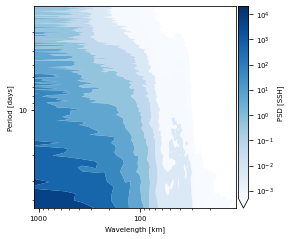
\includegraphics[trim={0 13mm 22mm 5mm},clip, width=2.3cm,height=2cm]{figures/plots/orca025_train_psd_spacetime.png} &
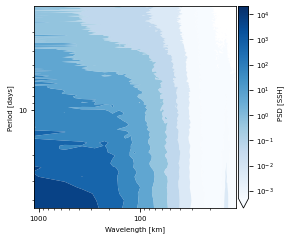
\includegraphics[trim={13mm 13mm 22mm 5mm},clip, width=2cm,height=2cm]{figures/plots/glorys12-f_train_psd_spacetime.png} &
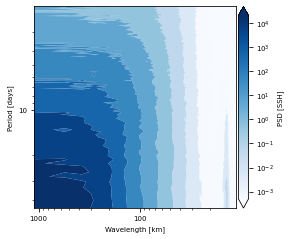
\includegraphics[trim={13mm 13mm 22mm 5mm},clip, width=2cm,height=2cm]{figures/plots/glorys12-r_train_psd_spacetime.png} &
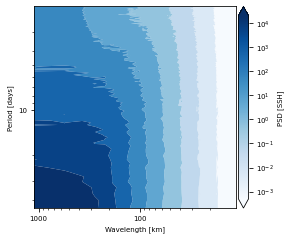
\includegraphics[trim={13mm 13mm 22mm 5mm},clip, width=2cm,height=2cm]{figures/plots/natl60_train_psd_spacetime.png} &
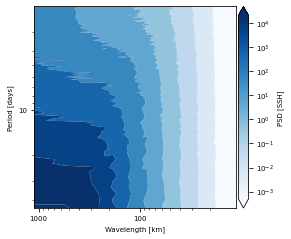
\includegraphics[trim={13mm 13mm 22mm 5mm},clip, width=2cm,height=2cm]{figures/plots/enatl60-t_train_psd_spacetime.png} &
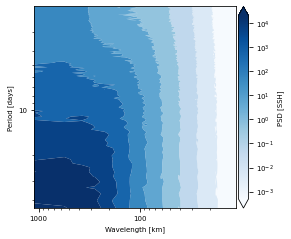
\includegraphics[trim={13mm 13mm 22mm 5mm},clip, width=2cm,height=2cm]{figures/plots/enatl60-0_train_psd_spacetime.png} &
 \\
%\vspace{3mm}
%%%%% GLORYS12-f %%%%%%%%

\hspace{0cm}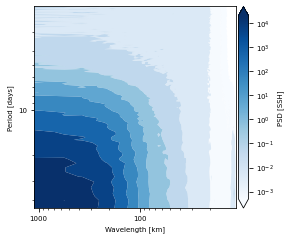
\includegraphics[trim={0mm 0 22mm 5mm},clip, width=2.3cm,height=2.3cm]{figures/plots/orca025_rec_psd_spacetime.png} &
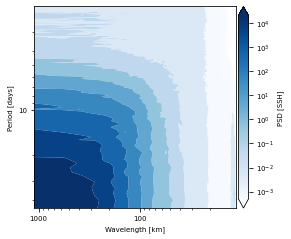
\includegraphics[trim={13mm 0 22mm 5mm},clip, width=2cm,height=2.3cm]{figures/plots/glorys12-f_rec_psd_spacetime.png}&
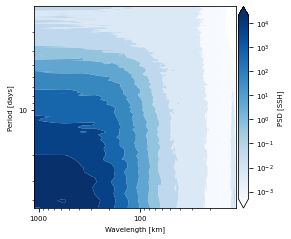
\includegraphics[trim={13mm 0 22mm 5mm},clip, width=2cm,height=2.3cm]{figures/plots/glorys12-r_rec_psd_spacetime.png}&
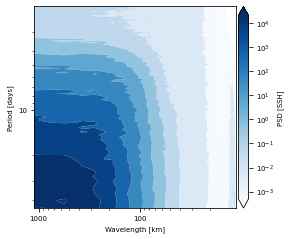
\includegraphics[trim={13mm 0 22mm 5mm},clip, width=2cm,height=2.3cm]{figures/plots/natl60_rec_psd_spacetime.png}&
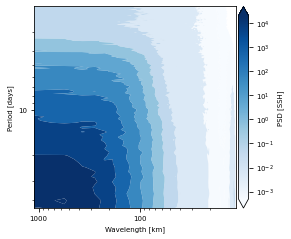
\includegraphics[trim={13mm 0 22mm 5mm},clip, width=2cm,height=2.3cm]{figures/plots/enatl60-t_rec_psd_spacetime.png} &
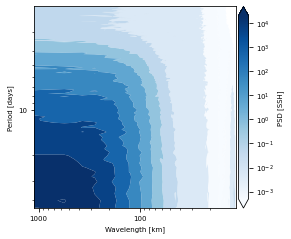
\includegraphics[trim={13mm 0 22mm 5mm},clip, width=2cm,height=2.3cm]{figures/plots/enatl60-0_rec_psd_spacetime.png}  &
\\

\end{tabular}
% \caption{Row I - Isotrophic PSD. Row 2 - Isotrophic PSD Score}
\caption{
Space-time spectral densities of the training datasets (first row) and their associated reconstructions (second row)} \vspace{-5mm}
\label{fig:spacetime_psd}
\end{center}

\end{subfigure}
\end{minipage}
\hspace{1.5cm}\begin{minipage}{0.01\linewidth}
\vspace{-1cm}

\begin{subfigure}[t]{.9\linewidth}
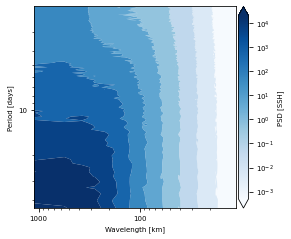
\includegraphics[trim={8.4cm 0 0 0},clip, width=0.8cm,height=2.3cm]{figures/plots/enatl60-0_train_psd_spacetime.png}
\end{subfigure}
\end{minipage}
\end{figure}

\begin{figure}[H]
\small
\begin{center}
\setlength{\tabcolsep}{1pt}
\begin{tabular}{ccc}

\hspace{3mm} Training PSD & 
\hspace{3mm} Reconstruction PSD & 
\hspace{3mm} PSD Score  \\

%\vspace{-2mm}
%%%%% ORCA025 %%%%%%%%

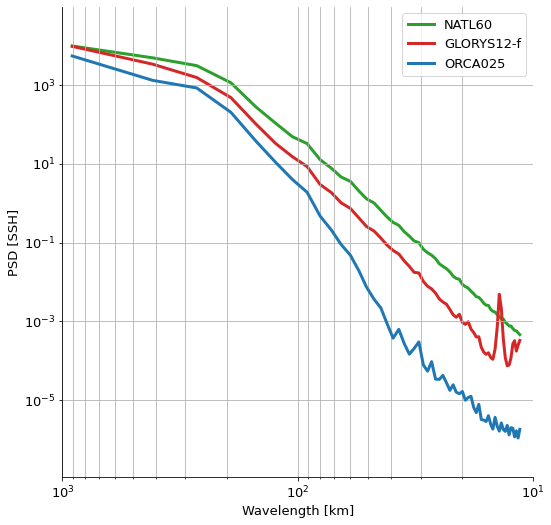
\includegraphics[width=0.32\textwidth]{figures/plots/isotrop_psd_res_train.png} &
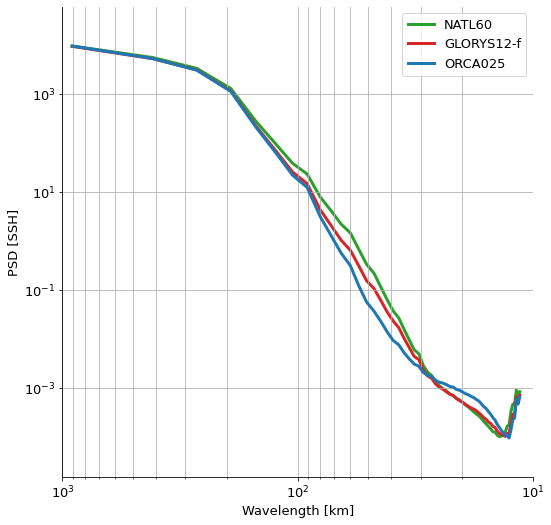
\includegraphics[width=0.32\textwidth]{figures/plots/isotrop_psd_res_rec.png} &
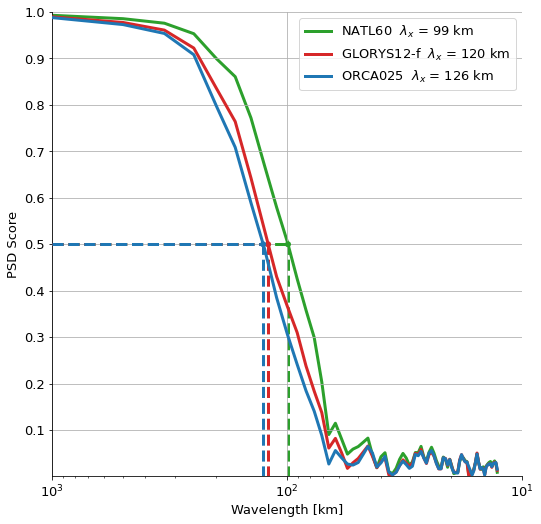
\includegraphics[width=0.32\textwidth]{figures/plots/res_1d_psd_score.png}


\end{tabular}
\vspace{-3mm}
% \caption{Row I - Isotrophic PSD. Row 2 - Isotrophic PSD Score}
\caption{
Spatial Power spectrum densities of the training dataset (left plot), reconstructed SSH field (center plot) as well as the associated PSD score (right plot)}\vspace{-5mm}
\label{fig:respsd}
\end{center}
\end{figure}


In this Section we look in more detail the impact of ocean run resolution in the training data and reconstructed fields. Looking at quantitative metrics in Table \ref{tab:benchmark_4dvarnet} we see the expected trend that using a higher resolution grid in the ocean run simulation enables a better outcome. However one might not have expected the training on the ORCA025 training that clearly contained fewer fine scale structures an weaker gradients to perform this well. Indeed when comparing at the training and reconstructed quantities in Figures \ref{fig:train_summer} \ref{fig:res_fields} we see that the observed quantities now exhibit minimal differences in magnitudes, effectively erasing the variations in the training data.
Qualitative differences can however been seen in the relative vorticity fields where residual artifacts due to the altimetry tracks can be seen (60°W, 39°N) for the two lower resolution training. This can be explained through Figure \ref{fig:res_train_psd} where we can see the power spectrum density of the observations used for training in the three cases compared with the one used for inference. We can see how the lower the resolution the bigger the gap between the training and testing energy levels. For the NATL60 training, the model has been trained on realistic energy levels whereas the GLORYS12 and ORCA025 models were trained on weaker altimetry tracks. When prompted to interpolate tracks with higher energy levels, they were able to extrapolate the energy but it induced artifacts around the input tracks. 
We can also note that the strain magnitude looks smoother for the NATL60 training and that the ORCA025 training doesn't show as much small structures in the Okubo-Weiss parameter and strain magnitude as the other two. 
When looking at the spatial power spectrum densities in Fig. \ref{fig:res_isotrop} of the stream function we can once again observe the similarity of the energy levels of the spatial PSD of the SSH. We can also note how the differences increase with derived quantities with higher energy for higher resolution in the training data.
Looking at the temporal PSD in Fig. \ref{fig:res_time_psd} however we see more significant difference with an order of magnitude between the NATL60 and other training around the 1 week wavelength. 

\begin{figure}[H]

\small
\begin{center}
\setlength{\tabcolsep}{1pt}
\begin{tabular}{ccc}

\hspace{3mm} Training PSD & 
\hspace{3mm} Reconstruction PSD & 
\hspace{3mm} PSD Score  \\

%\vspace{-2mm}
%%%%% ORCA025 %%%%%%%%

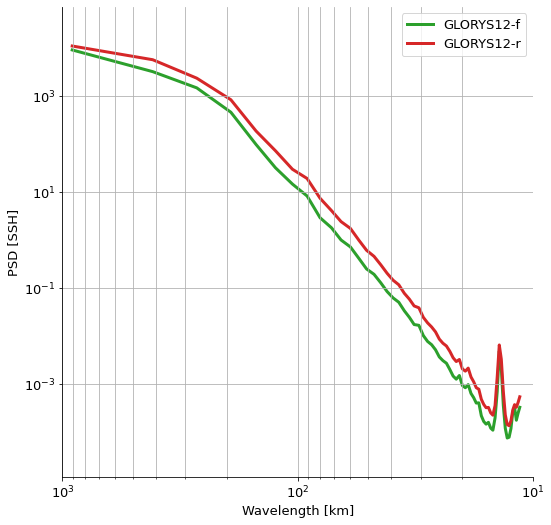
\includegraphics[width=0.32\textwidth]{figures/plots/isotrop_psd_rea_train.png} &
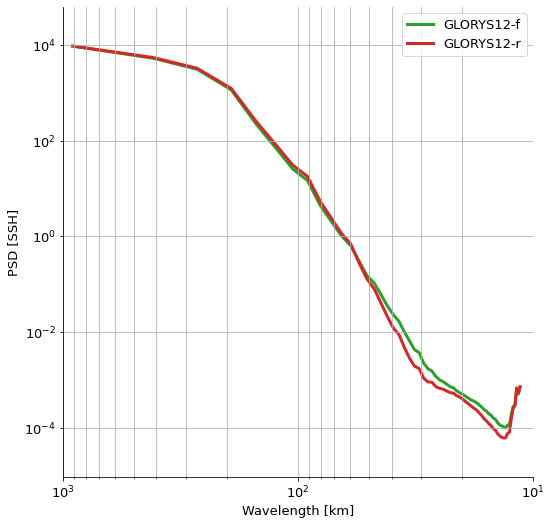
\includegraphics[width=0.32\textwidth]{figures/plots/isotrop_psd_rea_rec.png} &
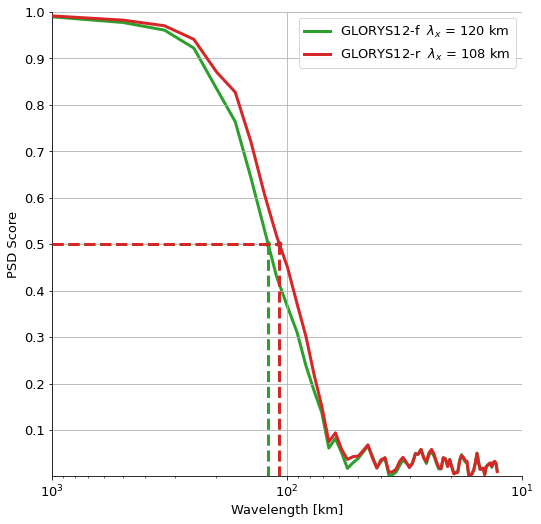
\includegraphics[width=0.32\textwidth]{figures/plots/rea_1d_psd_score.png}


\end{tabular}
\vspace{-3mm}
% \caption{Row I - Isotrophic PSD. Row 2 - Isotrophic PSD Score}
\caption{
Spatial Power spectrum densities of the training dataset (left plot), reconstructed SSH field (center plot) as well as the associated PSD score (right plot)}\vspace{-5mm}
\label{fig:reapsd}
\end{center}
\end{figure}

\subsection{Reanalysis}
\label{ssec:reanalysis}
Overall the reanalysis has similar effects as increasing the grid resolution:
\begin{itemize}
    \item It adds energy in the SSH field, and induce stronger gradients and vorticity fields.
    \item It improves the overall reconstruction metrics of the trained 4DVarNet
    \item Brings closer the training and evaluation PSD of the input altimetry tracks
    \item Improves the reconstructed fields by reducing artifacts around the input observations
    \item Raise more significantly the temporal spectrum density at fine scales than the spatial density 
\end{itemize}

One difference that can be noted is that the spatial PSD of the Kinetic energy of the reconstruction remains mostly unchanged when training on the free run or reanalysis of Glorys12 whereas training on NATL60 increased the energy levels. 

\subsection{Tide Modeling}
\label{ssec:tide}
\begin{figure}[H]
\small
\begin{center}
\setlength{\tabcolsep}{1pt}
\begin{tabular}{ccc}

\hspace{3mm} Training PSD & 
\hspace{3mm} Reconstruction PSD & 
\hspace{3mm} PSD Score  \\

%\vspace{-2mm}
%%%%% Tide psd %%%%%%%%

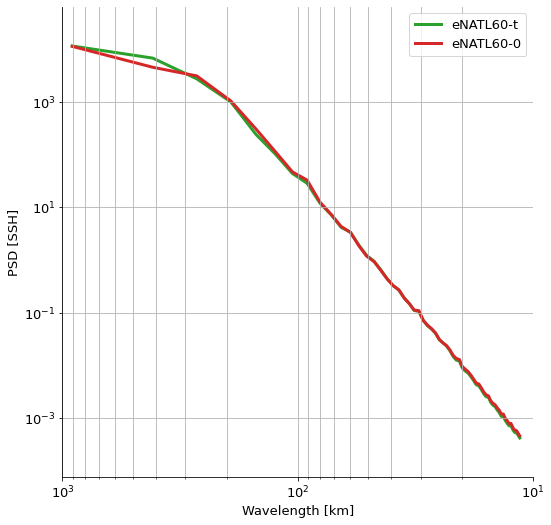
\includegraphics[width=0.32\textwidth]{figures/plots/isotrop_psd_tide_train.png} &
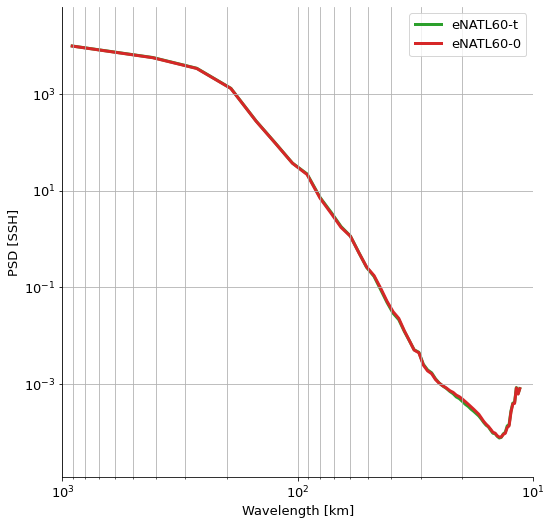
\includegraphics[width=0.32\textwidth]{figures/plots/isotrop_psd_tide_rec.png} &
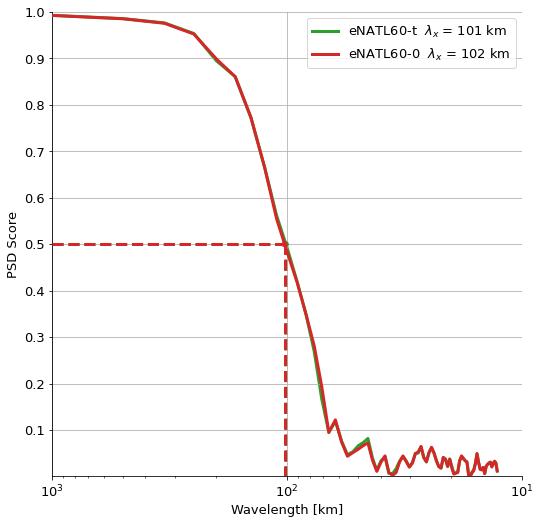
\includegraphics[width=0.32\textwidth]{figures/plots/tide_1d_psd_score.png}


\end{tabular}
\vspace{-3mm}
% \caption{Row I - Isotrophic PSD. Row 2 - Isotrophic PSD Score}
\caption{
Spatial Power spectrum densities of the training dataset (left plot), reconstructed SSH field (center plot) as well as the associated PSD score (right plot)}\vspace{-5mm}
\label{fig:tidepsd}
\end{center}
\end{figure}

We compare here the effect of explicit tide modeling in the training simulation. For this we use the eNATL60 simulation ran at 1/60°.  Contrary to other runs, those simulation contains barometric and wind forcing, we therefore remove the Dynamic Atmospheric Correction from the SSH fields. Additionally since the barotropic tides signal are removed from real altimetry tracks prior to interpolation, we also remove it from the training data by substracting the snapshot spatial mean over the training domain before calculating the daily averages.  

We find that training on those two dataset produce little differences in the reconstructions both quantitatively \ref{tab:benchmark_4dvarnet} and qualitatively in the fields (Fig. \ref{fig:tide_fields}) or in the spectral densities (Figs \ref{fig:tide_isotrop}, \ref{fig:tide_time_psd}, \ref{fig:tide_train_psd}). They both attain similar reconstruction metrics as the NATL60 training.
 
We identify two hypothesis linked to the lack of impact of explicit tide modeling:
\begin{itemize}
    \item The preprocessing applied on the training field and test altimetry tracks remove the main tide signals. We therefore effectively measure the impact of tide modeling in other ocean structures that may be less significant.
    \item The evaluation done in the geometry tracks may not capture the residual tide signals. New instruments like the KaRIN deployed in the SWOT mission may provide new ways to better quantify those effects.   
\end{itemize}

These findings provide motivation for carefully considering the purpose of the learning-based model when making decisions about the training data. Indeed In our case, explicitly modeling tide processes that are removed from the observations added overhead in the computational cost of running the simulation as well as in the preprocessing of the training data and did not improves the final interpolation model.

On the other hand training on a simulation with tide could also be a way to reduce the processing steps on the observation data by being able to interpolate maps from observation containing the tide signals.


\section{Conclusion}
\label{sec:conclusion}
We've seen in this study that training machine learning models on simulations offers reliably good performance on real altimetry data mapping. Even a relatively coarse simulation like ORCA025 provide competitive results with current operational methods. We have shown that producing higher fidelity SSH fields using reanalysis or higher resolution model allows for increased performances of the trained model. This is an exciting result that shows the potential for training operational products from ocean simulations and how advances in ocean modeling in operational oceanography can be beneficial. The results shown here are limited to the interpolation problem on a regional domain but the robustness of the performance shown are encouraging for further developing these results using a bigger domain and other physical quantities.

%%outputs/2023-05-20/20-41-13

%  Numbered lines in equations:
%  To add line numbers to lines in equations,
%  \begin{linenomath*}
%  \begin{equation}
%  \end{equation}
%  \end{linenomath*}



%% Enter Figures and Tables near as possible to where they are first mentioned:
%
% DO NOT USE \psfrag or \subfigure commands.
%
% Figure captions go below the figure.
% Acronyms used in figure captions will be spelled out in the final, published version.

% Table titles go above tables;  other caption information
%  should be placed in last line of the table, using
% \multicolumn2l{$^a$ This is a table note.}
% NOTE that there is no difference between table caption and table heading in the final, published version
%
%----------------
% EXAMPLE FIGURES
%
% \begin{figure}
% \includegraphics{example.png}
% \caption{caption}
% \end{figure}
%
% Giving latex a width will help it to scale the figure properly. A simple trick is to use \textwidth. Try this if large figures run off the side of the page.
% \begin{figure}
% \noindent\includegraphics[width=\textwidth]{anothersample.png}
%\caption{caption}
%\label{pngfiguresample}
%\end{figure}
%
%
% If you get an error about an unknown bounding box, try specifying the width and height of the figure with the natwidth and natheight options. This is common when trying to add a PDF figure without pdflatex.
% \begin{figure}
% \noindent\includegraphics[natwidth=800px,natheight=600px]{samplefigure.pdf}
%\caption{caption}
%\label{pdffiguresample}
%\end{figure}
%
%
% PDFLatex does not seem to be able to process EPS figures. You may want to try the epstopdf package.
%

%
% ---------------
% EXAMPLE TABLE
%
% \begin{table}
% \caption{Time of the Transition Between Phase 1 and Phase 2$^{a}$}
% \centering
% \begin{tabular}{l c}
% \hline
%  Run  & Time (min)  \\
% \hline
%   $l1$  & 260   \\
%   $l2$  & 300   \\
%   $l3$  & 340   \\
%   $h1$  & 270   \\
%   $h2$  & 250   \\
%   $h3$  & 380   \\
%   $r1$  & 370   \\
%   $r2$  & 390   \\
% \hline
% \multicolumn{2}{l}{$^{a}$Footnote text here.}
% \end{tabular}
% \end{table}

%%%%%%%%%%%%%%%%%%%%%%%%%%%%%%%%%%%%%%%%%%%%%%%
% SIDEWAYS FIGURES and TABLES
% AGU prefers the use of {sidewaystable} over {landscapetable} as it causes fewer problems.
%
% \begin{sidewaysfigure}
% \includegraphics[width=20pc]{figsamp}
% \caption{caption here}
% \label{newfig}
% \end{sidewaysfigure}
%
%  \begin{sidewaystable}
%  \caption{Caption here}
% \label{tab:signif_gap_clos}
%  \begin{tabular}{ccc}
% one&two&three\\
% four&five&six
%  \end{tabular}
%  \end{sidewaystable}

%% If using numbered lines, please surround equations with \begin{linenomath*}...\end{linenomath*}
%\begin{linenomath*}
%\begin{equation}
%y|{f} \sim g(m, \sigma),
%\end{equation}
%\end{linenomath*}

%%% End of body of article

%%%%%%%%%%%%%%%%%%%%%%%%%%%%%%%%%%%%%%%%%%%%%%%
%% Optional Appendices go here
%
% The \appendix command resets counters and redefines section heads
%
% After typing \appendix
%
%\section{Here Is Appendix Title}
% will show
% A: Here Is Appendix Title
%
%\appendix
%\section{Here is a sample appendix}

%%%%%%%%%%%%%%%%%%%%%%%%%%%%%%%%%%%%%%%%%%%%%%%
% Optional Glossary, Notation or Acronym section goes here:
%
% Glossary is only allowed in Reviews of Geophysics
%  \begin{glossary}
%  \term{Term}
%   Term Definition here
%  \term{Term}
%   Term Definition here
%  \term{Term}
%   Term Definition here
%  \end{glossary}


%%%%%%%%%%%%%%%%%%%%%%%%%%%%%%%%%%%%%%%%%%%%%%%
% Acronyms
%% NOTE that acronyms in the final published version will be spelled out when used in figure captions.
%   \begin{acronyms}
%   \acro{Acronym}
%   Definition here
%   \acro{EMOS}
%   Ensemble model output statistics
%   \acro{ECMWF}
%   Centre for Medium-Range Weather Forecasts
%   \end{acronyms}


%%%%%%%%%%%%%%%%%%%%%%%%%%%%%%%%%%%%%%%%%%%%%%%
% Notation
%   \begin{notation}
%   \notation{$a+b$} Notation Definition here
%   \notation{$e=mc^2$}
%   Equation in German-born physicist Albert Einstein's theory of special
%  relativity that showed that the increased relativistic mass ($m$) of a
%  body comes from the energy of motion of the body—that is, its kinetic
%  energy ($E$)—divided by the speed of light squared ($c^2$).
%   \end{notation}




%%%%%%%%%%%%%%%%%%%%%%%%%%%%%%%%%%%%%%%%%%%%%%%
%
% DATA SECTION and ACKNOWLEDGMENTS
%
%%%%%%%%%%%%%%%%%%%%%%%%%%%%%%%%%%%%%%%%%%%%%%%

\section*{Open Research Section}
This section MUST contain a statement that describes where the data supporting the conclusions can be obtained. Data cannot be listed as ''Available from authors'' or stored solely in supporting information. Citations to archived data should be included in your reference list. Wiley will publish it as a separate section on the paper’s page. Examples and complete information are here:
https://www.agu.org/Publish with AGU/Publish/Author Resources/Data for Authors


\acknowledgments
Enter acknowledgments here. This section is to acknowledge funding, thank colleagues, enter any secondary affiliations, and so on.


%%%%%%%%%%%%%%%%%%%%%%%%%%%%%%%%%%%%%%%%%%%%%%%
% REFERENCES and BIBLIOGRAPHY
%
\bibliography{biblio}
% don't specify bibliographystyle
%
%%%%%%%%%%%%%%%%%%%%%%%%%%%%%%%%%%%%%%%%%%%%%%%

%\bibliography{ enter your bibtex bibliography filename here }



%Reference citation instructions and examples:
%
% Please use ONLY \cite and \citeA for reference citations.
% \cite for parenthetical references
% ...as shown in recent studies (Simpson et al., 2019)
% \citeA for in-text citations
% ...Simpson et al. (2019) have shown...
%
%
%...as shown by \citeA{jskilby}.
%...as shown by \citeA{lewin76}, \citeA{carson86}, \citeA{bartoldy02}, and \citeA{rinaldi03}.
%...has been shown \cite{jskilbye}.
%...has been shown \cite{lewin76,carson86,bartoldy02,rinaldi03}.
%... \cite <i.e.>[]{lewin76,carson86,bartoldy02,rinaldi03}.
%...has been shown by \cite <e.g.,>[and others]{lewin76}.
%
% apacite uses < > for prenotes and [ ] for postnotes
% DO NOT use other cite commands (e.g., \citet, \citep, \citeyear, \nocite, \citealp, etc.).
%



\end{document}



More Information and Advice:

%%%%%%%%%%%%%%%%%%%%%%%%%%%%%%%%%%%%%%%%%%%%%%%
%
%  SECTION HEADS
%
%%%%%%%%%%%%%%%%%%%%%%%%%%%%%%%%%%%%%%%%%%%%%%%

% Capitalize the first letter of each word (except for
% prepositions, conjunctions, and articles that are
% three or fewer letters).

% AGU follows standard outline style; therefore, there cannot be a section 1 without
% a section 2, or a section 2.3.1 without a section 2.3.2.
% Please make sure your section numbers are balanced.
% ---------------
% Level 1 head
%
% Use the \section{} command to identify level 1 heads;
% type the appropriate head wording between the curly
% brackets, as shown below.
%
%An example:
%\section{Level 1 Head: Introduction}
%
% ---------------
% Level 2 head
%
% Use the \subsection{} command to identify level 2 heads.
%An example:
%\subsection{Level 2 Head}
%
% ---------------
% Level 3 head
%
% Use the \subsubsection{} command to identify level 3 heads
%An example:
%\subsubsection{Level 3 Head}
%
%---------------
% Level 4 head
%
% Use the \subsubsubsection{} command to identify level 3 heads
% An example:
%\subsubsubsection{Level 4 Head} An example.
%
%%%%%%%%%%%%%%%%%%%%%%%%%%%%%%%%%%%%%%%%%%%%%%%
%
%  IN-TEXT LISTS
%
%%%%%%%%%%%%%%%%%%%%%%%%%%%%%%%%%%%%%%%%%%%%%%%
%
% Do not use bulleted lists; enumerated lists are okay.
% \begin{enumerate}
% \item
% \item
% \item
% \end{enumerate}
%
%%%%%%%%%%%%%%%%%%%%%%%%%%%%%%%%%%%%%%%%%%%%%%%
%
%  EQUATIONS
%
%%%%%%%%%%%%%%%%%%%%%%%%%%%%%%%%%%%%%%%%%%%%%%%

% Single-line equations are centered.
% Equation arrays will appear left-aligned.

Math coded inside display math mode \[ ...\]
 will not be numbered, e.g.,:
 \[ x^2=y^2 + z^2\]

 Math coded inside \begin{equation} and \end{equation} will
 be automatically numbered, e.g.,:
 \begin{equation}
 x^2=y^2 + z^2
 \end{equation}


% To create multiline equations, use the
% \begin{eqnarray} and \end{eqnarray} environment
% as demonstrated below.
\begin{eqnarray}
  x_{1} & = & (x - x_{0}) \cos \Theta \nonumber \\
        && + (y - y_{0}) \sin \Theta  \nonumber \\
  y_{1} & = & -(x - x_{0}) \sin \Theta \nonumber \\
        && + (y - y_{0}) \cos \Theta.
\end{eqnarray}

%If you don't want an equation number, use the star form:
%\begin{eqnarray*}...\end{eqnarray*}

% Break each line at a sign of operation
% (+, -, etc.) if possible, with the sign of operation
% on the new line.

% Indent second and subsequent lines to align with
% the first character following the equal sign on the
% first line.

% Use an \hspace{} command to insert horizontal space
% into your equation if necessary. Place an appropriate
% unit of measure between the curly braces, e.g.
% \hspace{1in}; you may have to experiment to achieve
% the correct amount of space.


%%%%%%%%%%%%%%%%%%%%%%%%%%%%%%%%%%%%%%%%%%%%%%%
%
%  EQUATION NUMBERING: COUNTER
%
%%%%%%%%%%%%%%%%%%%%%%%%%%%%%%%%%%%%%%%%%%%%%%%

% You may change equation numbering by resetting
% the equation counter or by explicitly numbering
% an equation.

% To explicitly number an equation, type \eqnum{}
% (with the desired number between the brackets)
% after the \begin{equation} or \begin{eqnarray}
% command.  The \eqnum{} command will affect only
% the equation it appears with; LaTeX will number
% any equations appearing later in the manuscript
% according to the equation counter.
%

% If you have a multiline equation that needs only
% one equation number, use a \nonumber command in
% front of the double backslashes (\\) as shown in
% the multiline equation above.

% If you are using line numbers, remember to surround
% equations with \begin{linenomath*}...\end{linenomath*}

%  To add line numbers to lines in equations:
%  \begin{linenomath*}
%  \begin{equation}
%  \end{equation}
%  \end{linenomath*}



